\chapter{Theory}
\label{chapter:theory}
\epigraph{\textit{Wir wollen immer da hin, wo jeglicher Druck mal ein Ende hat
Ha'm immer tausend Sachen auf'm Zettel, sach' ma', kennst du das?}}{Deichkind}

\section{The Navier-Stokes equation}
\label{sec:navier_stokes_sec}
The starting point to study fluid dynamics is the Navier-Stokes equation~\cite{claude-louis-marie-henriMemoireLoisMouvement1827, stokesSteadyMotionIncompressible1848}, as motivated in Chap.~\ref{chapter:intro}.
Both Claude Navier in 1823 as well as Gorge G. Stokes in 1842 derived the momentum equation for a Newtonian liquid.
Historically these two were not the only ones. 
Siméon Denis Poisson and Barré de Saint-Venant came to the same conclusion around the same time~\cite{poissonNouvelleTheorieAction1831, de1843notea, jrHistoryAerodynamicsIts1998}.
But history is written and Navier as well as Stokes are identified with the derivation of the momentum of a fluid element. 

Mathematically the Navier-Stokes equation can be derived from one definition and two constraints.
The two constraints are mass and momentum conservation.
Mass conservation simply states that mass cannot be lost or created.
The same argument holds for the momentum.
By Noethers theorem every conserved quantity yields a symmetry and vice versa.
In this case conservation of momentum allows us to use the constraints on the solutions that translational symmetry requires.
Put simply a sliding drop experiment has to yield the same result in any laboratory on earths surface, independent of the exact location of the laboratory.
The last ingredient for the derivation is the definition of a fluid.
A fluid is ``\textit{a substance that flows and is not solid}`` according to the Cambridge Dictionary.
This definition can be refined, because a fluid is either a gas or a liquid that continuously deforms under shear stress, at least in the case of a Newtonian fluid.
And as such there is a linear relation between shear rate and shear velocity for a Newtonian fluid.
Clearly there are other liquids (which encloses granular systems to some extent) that exhibit different behaviour, for example toothpaste.
As long as there is no force applied to the tube the toothpaste does not flow.
Even the acceleration due to gravity when pointing the tube towards the ground does not exert enough force to generate a flow.
In contrast to Newtonian liquids those liquids have a different response function to shear, they can be addressed as \textit{power law} fluids.
While the phenomenology of these fluids, e.g., shear thinning or thickening, is very interesting and important in many industrial applications it is beyond the scope of this work. 
That said, in Chap.~\ref{chapter:second_paper} an extension towards more complex flows is presented. 
Instead of however changing the shear response we model thermal fluctuations to approximate the stochastic thin film equation (STF).
In fact, the step to derive an extension to our approach are nicely summarized in Chap.~\ref{chapter:second_paper}. 
It should serve as a guideline for further features, such as viscoelasticity for non-Newtonian liquids~\cite{bouchutNewModelShallow2013}. 

Knowing what a fluid is and taking into account the conservation of mass and momentum it is possible to derive the Navier-Stokes equation. 
By applying a continuity equation we assume that the fluid itself is a continuum and therefore ignore the underlying molecular structure for now. 
This allows us to describe the fluid state with a density $\rho(\mathbf{x},t)$, instead of describing every atom or molecule individually.
Assuming an infinitesimal small volume of fluid $V_0$ its density can only change if there is a flow through the boundaries of the volume $\partial V_0$,
\begin{equation}\label{eq:cont_1}
    \partial_t\int_{V_0}\rho\diff V = -\oint_{\partial V_0} \rho\vec{u}\cdot\diff \vec{A}, 
\end{equation}
where $\vec{u}(\vec{x},t)$ is the fluid's velocity, A is the area that encloses the volume $V_0$ and $\diff\vec{A}$ are the normals pointing outwards of the volume.
Violations of this Eq.~(\ref{eq:cont_1}) are equivalent to generation or destruction of mass.

Thanks to Gauss the integral over a closed surface can be written as divergence of a volume and thus the above equation becomes~\cite{koniglichegesellschaftderwissenschaftenzugottingenCommentationesSocietatisRegiae1811}
\begin{equation}\label{eq:cont_2}
    \partial_t\int_{V_0}\rho\diff V = -\int_{V_0} \vec{\nabla}\cdot(\rho\vec{u}) \diff V. 
\end{equation}
Since both sides are integrals over the volume $V_0$ we drop them and work with the differential equation
\begin{equation}\label{eq:cont_3}
    \partial_t\rho + \vec{\nabla}\cdot(\rho\vec{u}) = 0,
\end{equation}
which will be addressed as the continuity equation throughout the thesis.
Actually one finds this equation not only in fluid dynamics for mass conservation but as well in electrodynamics for charge conservation, where the second term is often referred to as flux~\cite{jacksonClassicalElectrodynamics2021, griffithsIntroductionElectrodynamics2013}.

For the momentum equation the same line of arguments is applied, however momentum can change for different reasons.
Momentum can for example be advected with the flow from or into the volume $V_0$.
Pressure on the other hand can be a source of momentum change and of course forces that are applied to the fluid are as well sources~\cite{krugerLatticeBoltzmannMethod2017}.
Collecting these terms and writing down an equation for the momentum we have,
\begin{equation}\label{eq:navier_stokes_1}
    \partial_t \int_{V_0}\rho\vec{u}\diff V = -\oint_{\partial V_0}(\rho\vec{u}\vec{u})\cdot\diff\vec{A} - \oint_{\partial V_0} p\diff\vec{A} + \int_{V_0} \vec{F}\diff V, 
\end{equation}
where $\vec{u}\vec{u}$ is used to denote the outer product
\begin{equation}
    \vec{u}\vec{u} = \begin{bmatrix}
    u_x u_x & u_x u_y & u_x u_z \\
    u_y u_x & u_y u_y & u_y u_z \\
    u_z u_x & u_z u_y & u_z u_z
    \end{bmatrix} .
\end{equation}
Using the divergence theorem again to reformulate everything in terms of volume integrals and dropping the integration the above equation becomes
\begin{equation}\label{eq:navier_stokes_2}
    \partial_t(\rho\vec{u}) = -\vec{\nabla}\cdot(\rho\vec{u}\vec{u}) - \vec{\nabla} p + \vec{F}.
\end{equation}
This however is not yet the Navier-Stokes equation, in fact this is the Euler equation~\cite{batchelorIntroductionFluidDynamics1967}.
In the derivation there is one term missing, because the momentum of a fluid can also change due to internal friction, or put simply, due to viscosity.
These viscous contributions are collected in the viscous stress tensor $\hat{\sigma}$ as
\begin{equation}\label{eq:stress_tens}
    \hat{\sigma}_{\alpha\beta} = \mu\left(\frac{\partial u_{\alpha}}{\partial x_{\beta}} + \frac{\partial u_{\beta}}{\partial x_{\alpha}}\right) + \lambda\delta_{\alpha\beta}\frac{\partial u_{\gamma}}{\partial x_{\gamma}}.
\end{equation}
This tensor introduces a lot of the complexity to the Navier-Stokes equation as in principle neither $\mu$ nor $\lambda$ need to be constants and in fact they are tensors themselves.

For the sake of clarity however here it is assumed that both $\mu$ and $\lambda$ are constants.
Inclusion of pressure to $\hat{\sigma}$ yields the total stress tensor $\tilde{\sigma}$. 
Due to symmetries of the problem there are various constraints on this tensor.
A fluid element can be rotated similar to a solid body, but it can also be stretched. 
In contrast to a solid body a fluid element is allowed to deform.
Working out these constraints we find that the pressure has to be a diagonal term and thus
\begin{equation}\label{eq:total_stress}
    \tilde{\sigma}_{\alpha\beta} = - p \delta_{\alpha\beta} + \mu\left(\frac{\partial u_{\alpha}}{\partial x_{\beta}} + \frac{\partial u_{\beta}}{\partial x_{\alpha}}\right) + \lambda\delta_{\alpha\beta}\frac{\partial u_{\gamma}}{\partial x_{\gamma}}.
\end{equation}
Now to get from the Euler equation (Eq.~(\ref{eq:navier_stokes_2})) to the Navier-Stoke we add the viscous stress tensor and rearrange terms,
\begin{equation}\label{eq:navier_stokes_3}
    \partial_t(\rho\vec{u}) + \vec{\nabla}\cdot(\rho\vec{u}\vec{u}) = - \vec{\nabla} p + \vec{\nabla}\left[\mu(\vec{\nabla}\vec{u} + \vec{\nabla}\vec{u}^T) + \left(\eta-\frac{2\mu}{3}\right)\vec{\nabla}\cdot\vec{u}\right] + \vec{F},
\end{equation}
where we have used the differential form of Eq.~(\ref{eq:total_stress}) and $\lambda = \eta - 2/3\mu$.

Instead of trying to solve this straight away, let's first discuss what we try to archive.
The main goal of this thesis is to model the dynamics of thin film flows.
An area of fluid dynamics usually addressed as creeping flows. 
The flow velocities in this regime are in fact much slower than the speed of sound $c_s$ ($c_s^{\ce{H2O}} \approx 1500m/s $). 
This allows for the simplification of an incompressible medium.
For such media or fluids one can assume that $\rho = const.$ and therefore by Eq.~(\ref{eq:cont_3}) 
\begin{equation}\label{eq:incomp}
    \vec{\nabla}\cdot\vec{u} = 0.
\end{equation}
A note of caution: While a constant density ($\rho = const.$) does satisfy the incompressibility constraint it is not unique to the underlying thermodynamics.
The thermodynamic compressibility $\kappa$ measures the change of volume with pressure and is given by 
\begin{equation}
    \kappa = \left(\frac{\partial V}{\partial p}\right)_T.
\end{equation}
Strictly speaking a fluid is incompressible as long as its density does not depend on the pressure $p$ or $\kappa = 0$.

Inserting this constraint Eq.~(\ref{eq:incomp}) into Eq.~(\ref{eq:navier_stokes_3}) yields therefore the Navier-Stokes equation for an incompressible fluid as
\begin{equation}\label{eq:navier_stokes_4}
    \rho(\partial_t\vec{u} + \vec{\nabla}\cdot\vec{u}\vec{u}) = - \vec{\nabla} p + \mu\Delta\vec{u} + \vec{F},
\end{equation}
where the symbol $\Delta$ denotes the Laplace operator ($\Delta f = \vec{\nabla}\cdot\vec{\nabla} f$).
The left hand side can be rewritten using the material derivative
\begin{equation}\label{eq:mat_dev}
    D_t = \partial_t + \vec{u}\cdot\vec{\nabla}, 
\end{equation}
which is a convenient measure for following a fluid element instead of a single point.
Inserting this, Eq.~(\ref{eq:navier_stokes_4}) can be written as
\begin{equation}\label{eq:navier_stokes_fin}
    \rho D_t \vec{u} =  - \vec{\nabla} p + \mu\Delta\vec{u} + \vec{F}.
\end{equation}
Eqs.~(\ref{eq:cont_3}, \ref{eq:navier_stokes_4}) cannot be solved because there are too few equations for too many unknowns.
So far there are five unknowns ($\rho, \mathbf{u}, p$) for four equations.
The clever way out of this misery is to use an equation of state that relates pressure, density, temperature, energy and entropy.
Especially the relation between pressure, density and temperature helps in closing the system of equations.
To define an equation of state is far from trivial.
It requires a thermodynamically consistent approach that is based on observations or theoretical assumptions.
The equation of state for an ideal gas was born from theoretical assumptions, e.g., non-interacting gas molecules, and reads~\cite{schwablStatisticalMechanics2006}
\begin{equation}\label{eq:eq_of_state}
    p = \rho R T,
\end{equation}
where $R$ is the specific gas constant and $T$ is the temperature.
Having a well defined state in the thermodynamical sense allows to relate pressure and density and therefore to close the system of equations.
The equation of state for an ideal gas, see Eq.~(\ref{eq:eq_of_state}), will be revisited in Chap.~\ref{chapter:method} where we discuss the lattice Boltzmann method.

The Navier-Stokes equation, see Eqs.~(\ref{eq:cont_3}, \ref{eq:navier_stokes_4}), offers a general framework to deal with fluid dynamics problems.
In the case of an incompressible non turbulent flow we have a solid understanding of the velocity field.
For compressible flows with developed turbulence on the other hand we still miss fundamental knowledge, as mentioned in Chap.~\ref{chapter:intro}.
This missing information is the reason that the automotive as well as aviation industry invests heavily in both real world experiments and CFD. 
For the concrete example of thin film flows, however, there is no need to ``solve'' the Navier-Stokes equation.
That is why in the next two sections different theories that build upon the Navier-Stokes are introduced.
Both of these theories using a scaling argument to severely simplify the resulting system of equations.

\section{Shallow water theory}
\label{sec:theory_shallow_water}
Solving the Navier-Stokes equation for the problems discussed in Chaps.~\ref{chapter:fourth_paper}-\ref{chapter:third_paper} is not needed.
Looking at Figs.~\ref{fig:examples_intro}-\ref{fig:morph_transition} one can identify that the height or thickness of the fluid layer is much smaller than the horizontal extension of the substrate.
This statement together with some more approximations allows to derive another system from the Navier-Stokes equation and the continuity equation which is called the shallow water or Saint-Venant equations~\cite{bTheorieMouvementNonpermanent1871}.

\subsection{Definition}
\begin{figure}
    \centering
    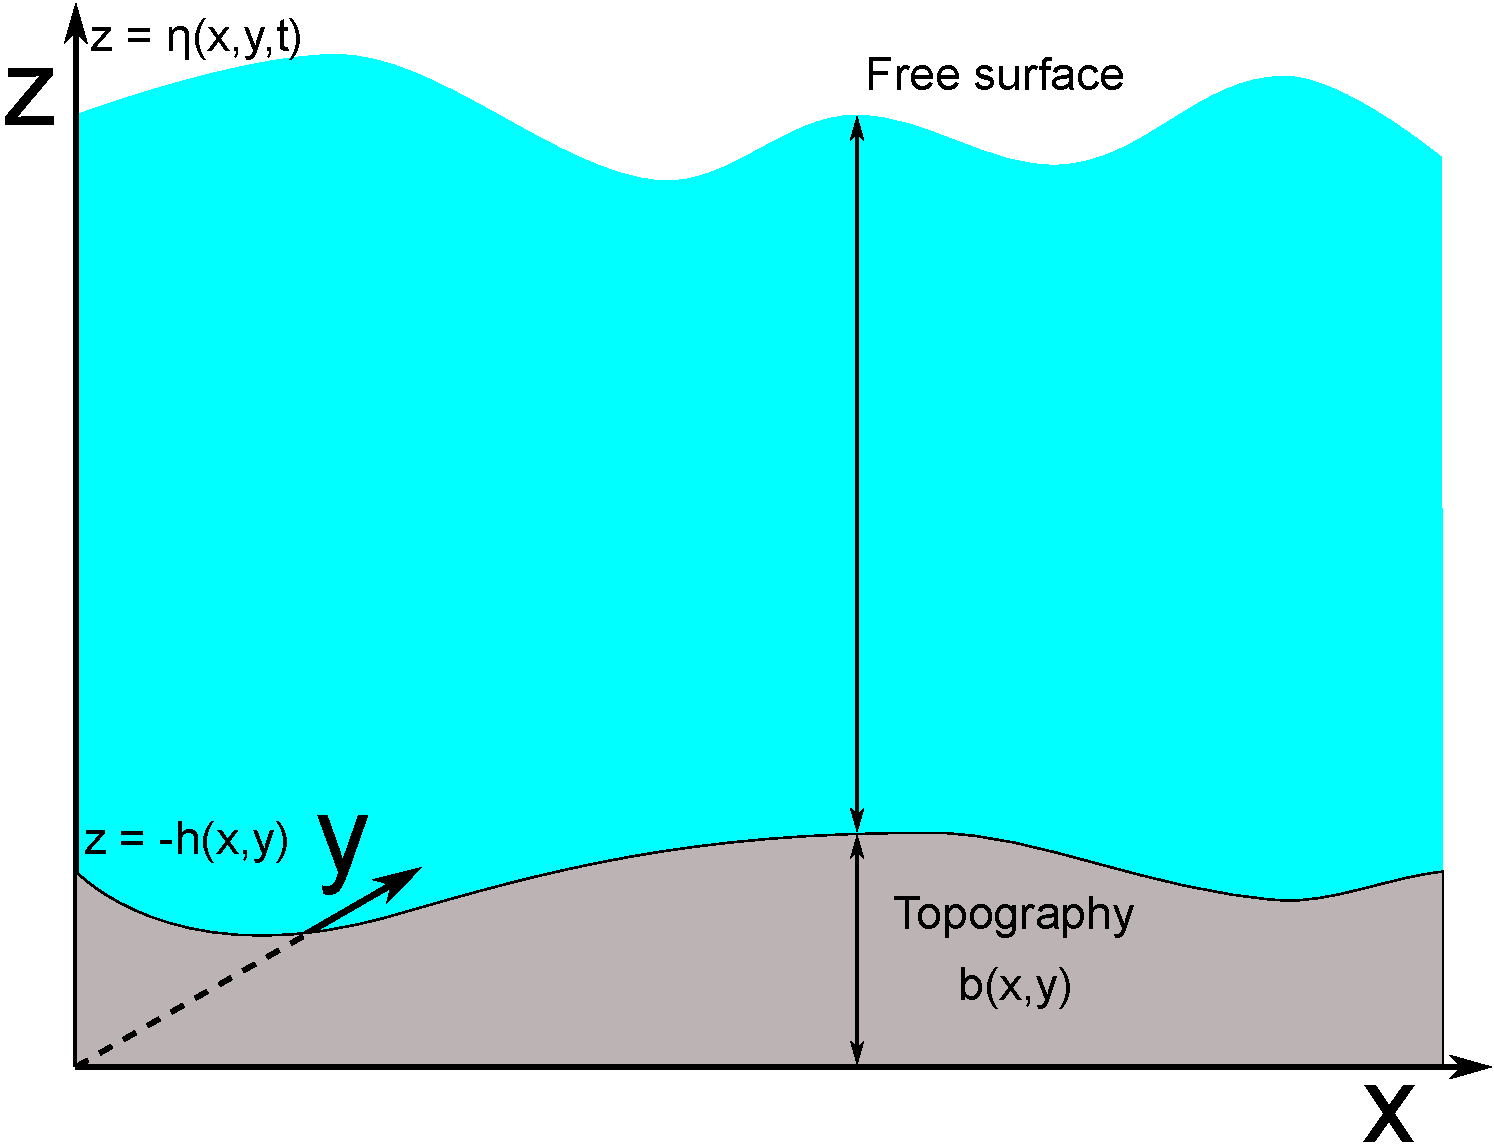
\includegraphics[width=0.55\textwidth]{graphics/simple_shallow_water.pdf}
    \caption{Schematic description of the shallow water problem. A liquid column with position of the free surface $\eta(x,y,t)$ covers a bottom topography $b(x,y)$.
    The liquid's height with the addition of the elevation of the topography defines the resulting height or z-component of the free surface.}
    \label{fig:shallow_water_drawing}
\end{figure}

The shallow water equations are a well working approximation to describe \textit{shallow} flows~\cite{tanShallowWaterHydrodynamics1992} and illustrated in Fig.~\ref{fig:shallow_water_drawing}.
``Shallow'' by definition of the Cambridge dictionary means ``\textit{having only a short distance from the top to the bottom}``, which in fact describes quite well what the model does.
Instead of having a fully resolved three-dimensional model of the fluid's density and velocity the shallow water approach assumes that the degrees of freedom in the vertical direction can be integrated out. 
Therefore all dynamics of the system are effectively captured by the evolution based on the horizontal degrees of freedom $(x,y)$.

Such strong assumptions require to take a look at the system at hand.
Coming back to the meaning of the word shallow, a shallow flow with a liquid column of height $h$ and horizontal length scale $L$ needs to satisfy
\begin{equation}\label{eq:thickness_length}
    \varepsilon := \frac{h}{L} \ll 1,
\end{equation}
where $\varepsilon$ is a measure for the difference between horizontal and vertical scales.
An illustrative example that satisfies this inequality is any of the three major oceans.
On average the oceans are about $3000m$ deep. 
They cover about $71\%$ of the earth's surface area which is approximately $361000000km^2$.
Dividing this number by three, to separate between Atlantic, Pacific and Indian ocean one gets a square with a side length of $~11000km$.
Inserting numbers in Eq.~(\ref{eq:thickness_length}) yields a ratio $\varepsilon \approx 3\cdot 10^{-4}$.
The average height of the fluid column is negligibly small as compared to its horizontal scales.
Therefore, the dynamics in the vertical direction can be considered instantaneous. 
The oceans are not the only dynamical system that with such a relation, the atmospheric layer also has a small $\varepsilon$. 
Atmospheric dynamics can be described with the shallow water model, at least to some extent.

Secondly comes the assumption of the pressure free surface.
Putting it simply, the shallow water model does not know what happens above the fluid.
The assumption is that the density of the layer above the fluid column is small when compared to the fluid density.
The oceans are mostly filled with water, the density of (salt) water is around a thousand times higher than the density of the air above ($\rho^{\ce{H2O}} \approx 1000$kg/m$^3$, $\rho^{\text{air}} \approx 1,25$kg/m$^3$).
To some extent this is, again, actually true for the atmospheric layer.
Using the barometric formula to relate the density with altitude,
\begin{equation}\label{eq:bareometric_form}
    \rho(h_1) = \rho(h_0)e^{-\frac{\Delta h}{h_s}},
\end{equation}
with $\Delta h = h_1 - h_0$ and $h_s = RT/Mg$ is the scale height.
Of course, the model can be refined with a so called multi layer approach~\cite{tubbsMultilayerShallowWater2009, prestininziEffectIntrinsicViscosity2013}, but by definition the assumption is that the upper end of the fluid column does not feel any pressure from above~\cite{tanShallowWaterHydrodynamics1992, jamesNewFrictionModel2019}.

Third, the horizontal velocity of the fluid has to vanish at the ``solid'' ground, or in terms of Fig.~\ref{fig:shallow_water_drawing} looking down from the free surface at $-h(x,y)$.
Although there is a viscosity associated with the fluid, friction with the bottom topography is the dominating dissipation channel.
This kind of boundary condition has been introduced in Chap.~\ref{chapter:intro} is called \textbf{no-slip} boundary condition~\cite{richardsonNoslipBoundaryCondition1973, degennesFluidWallSlippage2002, salmonLatticeBoltzmannMethod1999}.
While this may seem counterintuitive because fluid has no problem to flow over yet dry surfaces, modelling wetting or the wet-dry transition is a complex task, as seen later in this chapter and in Chap.~\ref{chapter:first_paper}.
After all, a theoretical model which is defined as a set of partial differential equations cannot account for the true complexity of nature~\cite{scrivenPhysicsApplicationsDIP1988}.
We come back to the idea of the no-slip boundary condition in Sec.~\ref{sec:thin_films}.

The big circular flow systems in the oceans like the Gulf Stream have much larger velocity components in the horizontal directions as compared to the vertical one.  
This is actually crucial to know because in the following mathematical modelling it is taken into account and will allow for further reduction of complexity.
We therefore assume that the vertical velocity component is small as compared to the horizontal ones.

The task now is to make, Eq.~(\ref{eq:navier_stokes_4}), aware about these constraints.
Although this sounds straightforward partial differential equations are complex. 
They are one of the topics in mathematics where researchers are satisfied with the irritating result that an equation cannot be solved, an undesired outcome for most Physicists.
Nevertheless, to come up with consistent strategies to solve them one can classify them, e.g., hyperbolic, parabolic, linear, nonlinear, initial value problem or boundary value problem.
There is in fact overlap between those terms, however to keep things simple it is sufficient to talk about initial or boundary value problems.
The former can be solved knowing the initial configuration which then defines the evolution, e.g., the initial coordinates and velocity of a pendulum. 
For the latter ones it is mandatory to know the solution at the boundaries. 
If we know the current temperature distribution on a metallic plate and the heat flux on the boundaries then we are able to calculate the temperature field on that plate at later times.
The shallow water system can be derived from the Navier-Stokes equation using both well defined boundary conditions and system specific approximations.
For example the statement \textit{pressure free surface} translates to the fact that there is a boundary condition requiring $p = 0$ at $z = \eta$. 
Therefore no pressure is acting on liquids interface.

\subsection{Scaling analysis}
\label{subssec:scaling_shallow water}
Starting with the system specific approximations, in Eq.~(\ref{eq:thickness_length}) a so-called scaling parameter $\varepsilon$ has been introduced. 
We use this parameter to rescale the velocities according to
\begin{equation}\label{eq:vel_scaling}
    u_x = \tilde{u}_x,\quad u_y = \tilde{u}_y,\quad u_z = \varepsilon\tilde{u}_z.
\end{equation}
For an incompressible fluid with vanishing density gradient Eq.~(\ref{eq:cont_3}) therefore becomes
\begin{equation}\label{eq:cont_nondim}
    \vec{\nabla}\cdot\vec{u} = \partial_x u_x + \partial_y u_y + \varepsilon\partial_z u_z = 0.
\end{equation}
To satisfy that all terms of this equation are the same order in $\varepsilon$ the coordinates need to be rescaled as well. 
This choice however is not unique and offers two possibilities~\cite{jamesNewFrictionModel2019}.
There is on the one hand the long wave approximation~\cite{oronLongscaleEvolutionThin1997},
\begin{equation}\label{eq:long_wave_scaling}
    x = \frac{\tilde{x}}{\varepsilon},\quad y = \frac{\tilde{y}}{\varepsilon},\quad z = \tilde{z},\quad t = \frac{\tilde{t}}{\varepsilon},
\end{equation}
which again is encountered in Sec.~\ref{subsec:thin_film_scaling} and has the effect of smoothing out spatial and temporal variations.
On the other hand is the thin layer scaling
\begin{equation}\label{eq:scaling_thin_layer}
    x = \tilde{x},\quad y = \tilde{y},\quad z = \varepsilon\tilde{z},\quad t = \tilde{t},
\end{equation}
which corresponds to the classical scaling of boundary layer theory~\cite{milne-thomsonTheoreticalHydrodynamics1996}.

In Eqs.~(\ref{eq:vel_scaling}-\ref{eq:scaling_thin_layer}) there is no distinct difference between both horizontal dimensions $(x,y)$. 
For the sake of clarity and to simplify the derivation of the shallow water model we neglect the $y$-components.
Of course, to study large oceanic systems or Coriolis forces one needs both horizontal dimensions, see e.g.,~\cite{dellarShallowWaterEquations2005, marcheDerivationNewTwodimensional2007}, but for the following derivation it is sufficient to use only one.
Furthermore we use Eq.~(\ref{eq:long_wave_scaling}), which represents long wave theory or scaling. 
We make use of this approach once more in the derivation of the thin film equation.
The benefit of this choice is the smoothing effect on variations which makes them more gradual. 
But not only the gradients in horizontal dimensions are multiplied with $\varepsilon^{-1}$.
The time is scaled with $\varepsilon^{-1}$ as well which smears the dynamics.
Inserting Eqs.~(\ref{eq:vel_scaling},\ref{eq:long_wave_scaling}) into Eq.~(\ref{eq:cont_3}) yields
\begin{equation}\label{eq:rescaled_cont}
    \tilde{\nabla}\cdot\tilde{\mathbf{u}} = \partial_{\tilde{x}} \tilde{u}_x + \partial_{\tilde{z}} \tilde{u}_z  = 0,
\end{equation}
where two dimensional vectors, such as $\mathbf{u} = (u_x, u_z)$ are bold while three dimensional ones are denoted with an arrow symbol.

Scaling analysis and renormalization are key concepts in modern physics~\cite{yakhotRenormalizationGroupAnalysis1986, IntroductionQuantumField2018}.
One of the key concepts of this idea are symmetries, and therefore transformations under which a given state does not change.
Fluid dynamics to some extent admits a conformal symmetry.
The governing equations describe the flow through a nanotube as well as the circular currents in oceans~\cite{secchiMassiveRadiusdependentFlow2016, marcheDerivationNewTwodimensional2007}.
Some features however such as the drag on an airfoil do not simply scale with the size of the system.
Therefore while a miniaturised model may create enough lift force, simply scaling up the size is not sufficient to ensure enough lift.  
In the following it will be helpful to introduce dimensionless numbers~\cite{ruzickaDimensionlessNumbers2008,neversFluidMechanicsChemical2019}.
These numbers have a long history in fluid dynamics.
The Reynolds number for example is a measure if a flow is turbulent or not, it depends only on proportions and not on an exact experiment.
With the knowledge of these number comparing experiments is straightforward, even if the experiments differ in many aspects.
The two dimensionless numbers of interest for the shallow water theory are the Reynolds number and the Froude number
\begin{equation}\label{eq:Re_and_Fr}
    Re = \frac{\rho L v_0}{\mu},\quad Fr = \frac{v_0}{\sqrt{g L}},
\end{equation}
where $L$ is a characteristic length scale of the problem, e.g., the mean water depth, $v_0$ and $g$ are a characteristic velocity and the gravitational acceleration ($g = 9.81 m/s^2$), respectively.
A characteristic velocity can be for example the inflow velocity from a boundary, or the speed of a certain wave type such as a tsunami.
Both numbers measure the magnitude of certain effects, in the case of the Reynolds number the inertial forces are compared against viscosity.
The Froude number is a measure to compare kinetic ($v_0$) with potential energy ($g L$).

In the next step both $Fr$ and $Re$ are used to make Eq.~(\ref{eq:navier_stokes_fin}) dimensionless.
For convenience the vector equation is split into two respective equations with gravity being the only force present.
Writing the full equation with all components yields
\begin{align}\label{eq:2d_RNS}
    \partial_t u_x + u_x\partial_x u_x + u_z\partial_z u_x &= -\partial_x p + \frac{1}{Re}\Delta u_x ,\\
    \partial_t u_z + u_z\partial_x u_x + u_z\partial_z u_z &= -\partial_z p - \frac{1}{Fr^2} + \frac{1}{Re}\Delta u_z ,
\end{align}
with the two dimensional Laplacian $\Delta = (\partial_x^2 + \partial_z^2)$.
Using long wave scaling, Eq.~(\ref{eq:long_wave_scaling}) and the rescaled length and time variables (e.g., $\tilde{x}$),
\begin{align}\label{eq:2d_RNS_eps}
    \varepsilon(\partial_{\tilde{t}} \tilde{u}_x + \tilde{u}_x \partial_{\tilde{x}} \tilde{u}_x + \tilde{u}_z \partial_{\tilde{z}} \tilde{u}_x ) &= -\varepsilon\partial_{\tilde{x}} \tilde{p} + \frac{1}{Re}(\varepsilon^2 \partial_{\tilde{x}}^2 \tilde{u}_x + \partial_{\tilde{z}}^2 \tilde{u}_x ) ,\\
    \varepsilon^2(\partial_{\tilde{t}} \tilde{u}_z + \tilde{u}_z\partial_{\tilde{x}} \tilde{u}_x + \tilde{u}_z\partial_{\tilde{z}} \tilde{u}_z) &= -\partial_{\tilde{z}}\tilde{p} - \frac{1}{Fr^2} + \frac{\varepsilon}{Re}(\varepsilon^2 \partial_{\tilde{x}}^2 \tilde{u}_z + \partial_{\tilde{z}}^2 \tilde{u}_z ) .
\end{align}
We now assume that terms with higher orders in $\varepsilon$ are negligible and therefore $O(\varepsilon^2) \rightarrow 0$, collecting only terms with up to $O(\varepsilon)$
\begin{align}\label{eq:2d_RNS_linear}
    \partial_{\tilde{t}} \tilde{u}_x + \tilde{u}_x\partial_{\tilde{x}} \tilde{u}_x + \tilde{u}_z\partial_{\tilde{z}} \tilde{u}_x &= -\partial_{\tilde{x}} \tilde{p} + \frac{\partial_{\tilde{z}}^2\tilde{u}_x}{\varepsilon Re}, \\
    0 &= -\partial_{\tilde{z}}\tilde{p} - \frac{1}{Fr^2} + \frac{\varepsilon\partial_{\tilde{z}}^2 \tilde{u}_z}{Re} .
\end{align}
Interestingly in the first of the two above equations the term associated to the horizontal viscosity is $O(\varepsilon^2)$ and can be dropped.
On the other hand with the assumption of the long wave scaling the second of the above equations yields the hydrostatic pressure, taking only $O(1)$ terms
\begin{equation}\label{eq:hydro_static}
    \partial_{\tilde{z}}\tilde{p} = -\frac{1}{Fr^2},
\end{equation}
which can be readily integrated, given $Fr$ is a constant, using the upper bound at the liquid air interface $\eta(x)$ 
\begin{equation}\label{eq:hydro_static_int}
    \tilde{p} = \frac{1}{Fr^2}(\tilde{\eta} - \tilde{z}).   
\end{equation}
This implies that $\partial_{\tilde{x}}p$ does not depend on $\tilde{z}$ and therefore states that the pressure gradient is conserved along z.

Summarizing the impact of the approximation, on the continuity equation Eq.~(\ref{eq:rescaled_cont}) and Eqs.~(\ref{eq:2d_RNS_linear}-\ref{eq:hydro_static}) and dropping the tilde we get 
\begin{align}
    \partial_x u_x + \partial_z u_z &= 0, \label{eq:cont_sw_euler}\\
    \partial_t u_x + u_x\partial_x u_x + u_z\partial_{z} u_x &= -\partial_x p + \frac{\partial_z^2 u_x}{\varepsilon Re}, \label{eq:mom_sw_euler}\\
    \partial_z p &= -\frac{1}{Fr^2} \left(+\frac{\varepsilon\partial_{\tilde{z}}^2 \tilde{u}_z}{Re}\right), \label{eq:hydrostat_sw_euler}
\end{align}
with the addition of boundary conditions at the liquid air interface ($z = \eta$)
\begin{align}
    \partial_t \eta + u_x\partial_x\eta - u_z &= 0, \label{eq:sw_boundaries_top_1}\\
    p &= 0, \label{eq:sw_boundaries_top_2}\\
    \partial_z u_x &= 0, \label{eq:sw_boundaries_top_3}
\end{align}
as well as the no slip condition at the liquid solid interface ($z = b$)
\begin{align}
    u_x = 0, \label{eq:no-slip_sw1}\\
    u_z = 0. \label{eq:no-slip_sw2}
\end{align}
One interesting limit is the case when $\varepsilon Re \rightarrow \infty$.
In this limit both the continuity equation as well as the boundary conditions are untouched.
The only part that is modified is the momentum equation Eq.~(\ref{eq:mom_sw_euler}),
\begin{equation}
    \partial_t u_x + u_x\partial_x u_x + u_z\partial_{z} u_x = -\partial_x p,
\end{equation}
which describes the hydrostatic Euler equations~\cite{brenierGeneralizedSolutionsHydrostatic2008}.

\subsection{Integration along the vertical dimension}
\label{subsec:int_sw}
The classical approach to obtain the shallow water equations is to integrate the system of Eqs.~(\ref{eq:cont_sw_euler}-\ref{eq:hydrostat_sw_euler}) along the vertical dimension.
Having already neglected the $y$-component, the integration will also integrate out degrees of freedom in $z$.
The resulting system will therefore only vary with a $x$ dependency.
Analogous to Fig.~\ref{fig:shallow_water_drawing} by integration along the vertical direction of the three dimensional density field $\rho$, the height of the fluid column emerges as a dynamic quantity,
\begin{equation}\label{eq:shallow_water_height}
    h(x) = \eta(x) - b(x).    
\end{equation}
Therefore it is a reduction of complexity and effectively enslaves the vertical dynamics to the horizontal one.

In terms of velocity a new variable needs to be defined which accounts for the averaging along the vertical
\begin{equation}\label{eq:sw_discharge}
    hU = \int_{b}^{\eta}u_x\diff z,
\end{equation}
where $h$ is the height (Eq.~(\ref{eq:shallow_water_height})) and $U$ the height averaged velocity. 
The pair $hU$, thus height that is transported with velocity $U$, can also be addressed as discharge $Q$~\cite{salmonLatticeBoltzmannMethod1999}.
Having introduced the height $h$ and the discharge $Q$ the next step is to integrate the continuity and momentum equations, Eqs.~(\ref{eq:cont_sw_euler}, \ref{eq:mom_sw_euler}). 
Starting with the former
\begin{align}
    0 =& \int_b^{\eta} (\partial_x u_x + \partial_z u_z) \diff z, \label{eq:vert_int_cont_1}\\
    =& \int_b^{\eta} (\partial_x u_x \diff z) + u_z|_{z = \eta} - u_z|_{z = b}, \label{eq:vert_int_cont_2}
\end{align}
 where the $z$ dependent velocity can be integrated. 
 For the $x$-component we make use of the integration rule of Leibniz, 
\begin{equation}\label{eq:int_leibniz}
    \partial_x\int_{A(x)}^{B(x)}F(x,y)\diff y = \int_{A(x)}^{B(x)}\frac{\partial F(x,y)}{\partial_x} \diff y + \frac{\diff B(x)}{\diff x}F(x,B(x)) - \frac{\diff A(x)}{\diff x} F(x, A(x)),
\end{equation}
which upon inserting yields
\begin{equation}\label{eq:vert_int_cont_3}
    0 = \partial_x\left(\int_{b}^{\eta} u_x \diff z \right) - u_x|_{z=\eta}\partial_x\eta + u_x|_{z=b}\partial_x b + u_z|_{z = \eta}  - u_z|_{z = b}. 
\end{equation}
Simplifying this equation by making use of Eq.~(\ref{eq:sw_boundaries_top_1}) and Eqs.~(\ref{eq:no-slip_sw1}-\ref{eq:no-slip_sw2}) yields
\begin{equation}\label{eq:vert_int_cont_4}
    0 = \partial_x\left(\int_{b}^{\eta} u_x \diff z \right) + \partial_t \eta,
\end{equation}
where the integral is simply the discharge $hU$. 
Assuming that the river or shallow water bed $b(x)$ is time independent the equation can be condensed to
\begin{equation}\label{eq:shallow_water_cont_true}
    \partial_t h + \partial_x(hU) = 0.
\end{equation} 
This is equal to the statement whenever height changes it has to flow somewhere and therefore ensures mass conservation. 
Rivers such as the Colorado River change their bed quite significantly with time, the same is true for coastlines as we know that they erode with time.
The reason we use $b(x)$ and not $b(x, t)$ is the mismatch in time scales between the erosion and the flow.
For example, the Grand Canyon is about 5-6 million years old and roughly 1.9km deep, the Colorado River flows however with a velocity of $\approx 3.5$km/h~\cite{grafColoradoRiverGrand1997}.

Performing the horizontal integration to the depth averaged momentum equation, see Eq.~(\ref{eq:mom_sw_euler}) we have
\begin{align}\label{eq:mom_shallow_water_int}
    \int_b^{\eta}\left(-\partial_x p + \frac{\partial_z^2 u_x}{\varepsilon Re}\right)\diff z &= \int_b^{\eta}\left(\partial_t u_x + u_x\partial_x u_x + u_z\partial_{z} u_x\right)\diff z. 
\end{align}
The two terms on the left hand side can be integrated straight away. 
We know that the pressure gradient $\partial_x p$ is conserved along the vertical dimension. 
The other term ($\propto\partial^2 u$) has a similar shape as the viscous term in Eq.~(\ref{eq:navier_stokes_4}). 
Performing the integral therefore yields
\begin{equation}\label{eq:sw_mom_left}
    \int_b^{\eta}\left(-\partial_x p + \frac{\partial_z^2 u_x}{\varepsilon Re}\right)\diff z = -h\partial_x p + \frac{\partial_z u_x|_{z = \eta} - \partial_z u_x|_{z=b}}{\varepsilon Re},
\end{equation}
with the boundary condition that fluid does not accelerate into the air phase, see Eq.~(\ref{eq:sw_boundaries_top_3}), the left hand side reduces to
\begin{equation}
    \int_b^{\eta}\left(-\partial_x p + \frac{\partial_z^2 u_x}{\varepsilon Re}\right)\diff z = -h\partial_x p - \frac{\partial_z u_x|_{z=b}}{\varepsilon Re}.
\end{equation}
The right hand side of Eq.~(\ref{eq:mom_shallow_water_int}) reads
\begin{align}\label{eq:mom_shallow_rhs}
    \int_b^{\eta}\left(\partial_t u_x + u_x\partial_x u_x + u_z\partial_{z} u_x\right)\diff z &= \int_b^{\eta}\left(\partial_t u_x\right)\diff z \nonumber\\
    &+ \int_b^{\eta}\left(u_x\partial_x u_x + u_z\partial_{z} u_x\right)\diff z ,
\end{align}
where the integral is split into two separate integrals for convenience.
The time dependent part can be easily integrated using Eq.(~\ref{eq:int_leibniz})
\begin{equation}\label{eq:first_term_rhs_mom_sw}
    \int_b^{\eta}\left(\partial_t u_x\right)\diff z = \partial_t \int_b^{\eta} u_x \diff z - \partial_t\eta u_x|_{z=\eta} - \partial_t b u_x|_{z=b} = \partial_t(hU) - \partial_t\eta u_x|_{z=\eta} - \partial_t b u_x|_{z=b}. 
\end{equation}
The other integral is somewhat more tricky.
First, the $u_z\partial_z u_x$ term is integrated by parts
\begin{equation}
    \int_b^{\eta}u_z(\partial_{z} u_x)\diff z = [u_x u_z]_b^{\eta} - \int_b^{\eta} (\partial_z u_z) u_x \diff z.
\end{equation}
We use this intermediate result, Eq.~(\ref{eq:cont_sw_euler}) and the integration rule of Leibnitz to perform the integral of the second line of Eq.(\ref{eq:mom_shallow_rhs}) 
\begin{align}
    \int_b^{\eta}(u_x\partial_x u_x &+ u_z\partial_{z} u_x )\diff z = 2\int_b^{\eta} u_x\partial_x u_x \diff z + [u_x u_z]_b^{\eta},\nonumber \\
     &= \partial_x\left(\int_b^{\eta}u_x^2 \diff z\right) + \partial_t\eta u_x|_{z=\eta} + u_x(u_x\partial_x b - u_z)|_{z=b},
\end{align}
where the same line of arguments as in Eq.~(\ref{eq:vert_int_cont_3}) has been used.
Applying the boundary condition to this equation and using the definition for height and discharge we have
\begin{equation}\label{eq:sw_mom_final}
    \partial_t(hU) + \partial_x(\beta hU^2) = -h\partial_x p - \tau_b,
\end{equation}
where two new variables appear.
The first one is the Boussinesq coefficient $\beta$ which is defined by the equation
\begin{equation}\label{eq:boussinesq}
    \int_b^{\eta} u_x^2 \diff z = \beta h U^2,
\end{equation}
and the second one is the friction or the shear stress at the bottom of the fluid column
\begin{equation}\label{eq:sw_bot_friction}
    \tau_b = \frac{\partial_z u_x|_{z=b}}{\varepsilon Re}. 
\end{equation}
Both $\beta$ as well as $\tau_b$ do depend on $u$. 
Therefore to know their exact contribution one needs to know about the flow.
Without the concrete knowledge of $u$ there is however one observation concerning Eq.~(\ref{eq:boussinesq})
\begin{equation}\label{eq:beta_lims}
    \beta = 1 + \frac{1}{h}\int_b^{\eta}\left(1 - \frac{u}{U}\right)^2 \diff z,
\end{equation}
and therefore $\beta \geq 1$.
To understand the implications of these terms we discuss an instructive example.

\begin{figure}
    \centering
    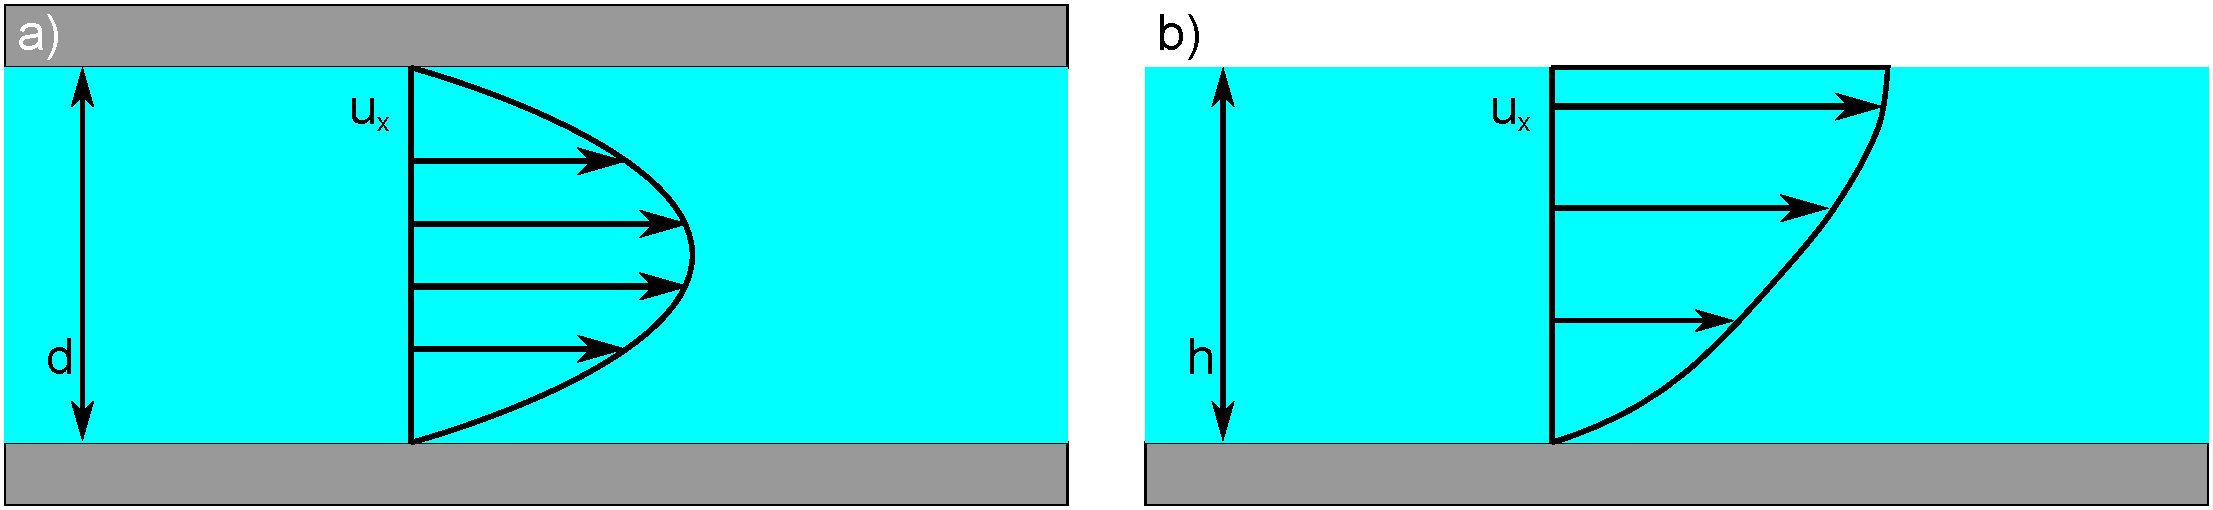
\includegraphics[width=0.95\textwidth]{graphics/Simple_flow.pdf}
    \caption{a) Schematic, cut through the center, velocity profile of a pipe flow with wall friction and no slip boundary condition.
    The flow velocity $u_x$ can be calculated using Eq.~(\ref{eq:pois_vel_profile}).
    b) Similar case in terms of a shallow water geometry. 
    The upper wall is replaced with a pressure free boundary while the lower wall induces friction according to a no-slip boundary condition.
    }
    \label{fig:pois_vel_profile}
\end{figure}
\subsection{Poiseuille flow}
The Poiseuille flow is one amongst those few problems that can be solved analytically~\cite{suteraHistoryPoiseuilleLaw}.
To have an idea about the flow, one can think of a circular pipe.
The pipe is fully filled with a (Newtonian) liquid, see Fig.~\ref{fig:pois_vel_profile} a) for an oversimplified illustration.
By an external pressure gradient, for example a pump, a continuous flow is generated.
The velocity profile of this flow can be explained with the equation~\cite{batchelorIntroductionFluidDynamics1967, krugerLatticeBoltzmannMethod2017}
\begin{equation}\label{eq:pois_vel_profile}
    u_x(y) = -\frac{\partial_x p}{2\mu}y(y-d),
\end{equation}
where $d$ is the diameter of the pipe.
The profile is parabolic with vanishing $u_x$ at the walls and a maximum at $d/2$. 
Thus the above equation defines the balance between the driving force, here the pressure difference, and the friction at the walls.

In Fig.~\ref{fig:pois_vel_profile} b) the flow is not enclosed between two boundaries but has a pressure free surface.
The solution is not anymore given by Eq.~(\ref{eq:pois_vel_profile}) but reduces to the half-Poiseuille or Nusselt solution with a new self similar quantity $\bar{h}$~\cite{jamesNewFrictionModel2019}
\begin{equation}\label{eq:bar_h}
    \bar{h} = \frac{z - b}{h}, \quad \frac{u}{U} = 3\left(\bar{h} - \frac{\bar{h}^2}{2}\right), 
\end{equation}
where $\bar{h}$ is constructed to be in the interval between 0 and 1.
Inserting $\bar{h}$ into Eq.~(\ref{eq:beta_lims}) reveals that the Boussinesq coefficient is given as $\beta = 6/5$, where the integration can be performed using a transformation of the integral measure.
The friction term Eq.~(\ref{eq:sw_bot_friction}) becomes 
\begin{equation}
    \tau_b = \frac{3}{\varepsilon Re}\frac{U}{h} .
\end{equation}
The friction term $\tau_b$ depends linearly on $U$ the mean flow velocity.
Interestingly for large Reynolds numbers the friction can become negligible, with the transition to the inviscid shallow water regime.

A word of caution is needed when using $\tau_b$.
Friction forces in real experiments are dependent on the actual boundary condition at $z = b$.
Both the topography and the specific type of material at the bottom will influence the measured value of $\tau_b$. 
By modelling a dissipative force such as friction we make an error, and a priori we do not know if that error is large or small.
It is therefore often simpler and more accurate to use data from empirical studies or real world experiments.
Within the shallow water literature an often encountered coefficient is the one of Manning, the empirical law that connects flow velocity with friction can be found in Ref.~\cite{f.asceOpenChannelHydraulics2021}.

To close this section we quickly collect the equations that form the shallow water system, see Eqs.~(\ref{eq:shallow_water_cont_true}, \ref{eq:sw_mom_final}).
The generalization of these equations towards a second horizontal dimension is straightforward and can be written as~\cite{salmonLatticeBoltzmannMethod1999, dellarNonhydrodynamicModesPriori2002, thommesLatticeBoltzmannMethods2007}
\begin{align}    
        \partial_t h &+ \nabla \cdot (h\mathbf{u}) = 0, \label{eq:shallow_water_01}\\
        \partial_t (h\mathbf{u}) + \nabla&\cdot (p \mathbb{1} + h\mathbf{u}\mathbf{u} - S) = 0, \label{eq:shallow_water_02} 
\end{align}
where $\mathbf{u} = (u_x, u_y)$ and the only unknown $\mathcal{S}$ is a yet undefined source term. 
The system Eqs.~(\ref{eq:shallow_water_01}-\ref{eq:shallow_water_02}) concludes the shallow water model. 
In Chap.~\ref{chapter:first_paper} we show how this translates into a numerical solver.

Following in this chapter are two more sections.
The next section and the main point of interest of this work is a short and phenomenological oriented derivation of the thin film model.
In the last section the chapter concludes with a comparison of shallow water with thin film theory.

\section{Lubrication theory and thin films}
\label{sec:thin_films}
Thin liquid films are an interesting problem to study.
Their dynamics is seemingly easy to explain but bares a lot of complexity.
Many of us have played with soap bubbles and experienced their bursting, which is essentially a free standing film thus there is no solid substrate.
Or have seen thin oil films on water puddles and their beautiful refraction patterns.
As already mentioned, coatings are a prime example for thin liquid films. 
Complexity is generated due to the shape of the equation that describes the thin film dynamics, usually a non linear forth order partial differential equation of the film thickness.
When the thickness of a film becomes small, e.g., only a few tens of nanometers the complexity can even be enhanced. 
Complex behaviour can arise due to thermal fluctuations or strictly speaking the mathematical unsolvable problem of moving contact lines e.g., when a wet to dry transition happens.
Similar to the above section's scaling argument and the long wave theory, the Navier-Stokes equation can be reduced to the thin film equation. 
Although with the difference to the shallow water system, see Eqs.~(\ref{eq:shallow_water_01}-\ref{eq:shallow_water_02}), that the thin film equation does only admit a continuity like equation and no accompanying momentum equation~\cite{oronLongscaleEvolutionThin1997, degennesWettingStaticsDynamics1985, crasterDynamicsStabilityThin2009}.

\begin{figure}
    \centering
    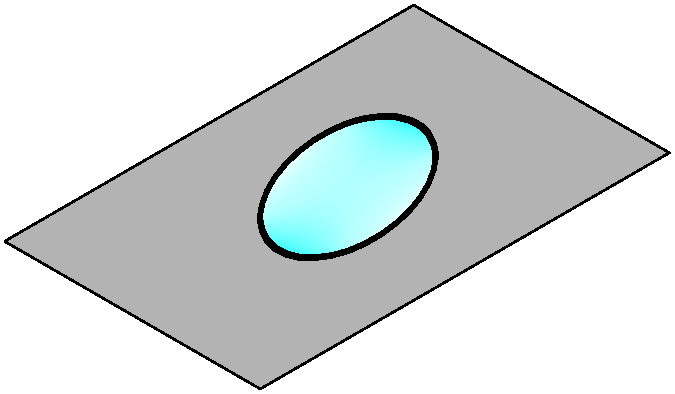
\includegraphics[width=0.95\textwidth]{graphics/contact_line.pdf}
    \caption{A liquid droplet placed on a smooth substrate.
    The three phase contact line which is the interface between the vapor, the solid and liquid phase is displayed as a thick black line.}
    \label{fig:contact_line_drop}
\end{figure}
Similar to the shallow water system, the thin film equation only considers the dynamics of a thin liquid \textit{layer}. 
In principle this layer can be unsupported, it can as well be placed on top of a yet undefined surface or substrate.
Within this thesis we consider exclusively supported thin films on substrates.
The defining equation that describes the dynamics of a thin liquid film can be written as~\cite{thielePatternedDepositionMoving2014, oronLongscaleEvolutionThin1997, crasterDynamicsStabilityThin2009, bonnWettingSpreading2009} 
\begin{equation}\label{eq:simple_thin_film}
    \partial_t h = \nabla\cdot\left(M(h)\nabla p\right).
\end{equation}
On the left hand side we have the change in thickness ($\partial_t h$), which can only be achieved by applying a pressure gradient ($\nabla p$).
In Eq.~(\ref{eq:simple_thin_film}) two unknowns are introduced.
The first one is the mobility $M(h)$ which determines the exact velocity boundary condition for $h=0$.
Using the no-slip boundary condition~\cite{beckerThinfilmEquationRecent2005}, see Eq.~(\ref{eq:no-slip_sw1}), we have 
\begin{equation}\label{eq:no-slip-mobility}
    M(h) = \frac{h^3}{3\mu},
\end{equation}
with $\mu$ being the (dynamic) viscosity. 
Therefore the mobility is inversely proportional to the viscosity.
Of course the velocity boundary condition can be relaxed which is often desired e.g., for contact line movement.

For problems such as dewetting it is actually a known approximation to relax the velocity boundary condition at the liquid solid interface~\cite{munchDewettingRatesThin2005, munchLubricationModelsSmall2005, fetzerNewSlipRegimes2005}.
Dewetting usually refers to an unstable film which by so-called film rupture recedes into separated droplets. 
Depending on the film's properties different modes of dewetting can be identified, such as spinodal dewetting or hole nucleation.
Film stability and the dewetting instability is a reoccurring topic throughout this thesis. 
Dewetting becomes less likely that thicker the film is, as a rule of thumb.
Thicker thin films usually tend to rupture via nucleation, while thinner films tend to rupture via spinodal dewetting.
Rupture and dewetting can also be caused by gradients, e.g., surface tension gradients or even thermal fluctuations.
The dynamics of a dewetting thin film depend heavily on the dynamics of the contact line. 

The term contact line or to be precise three-phase contact line defines the single one dimensional interface that connects all three phases involved in the problem, as displayed in Fig.~\ref{fig:contact_line_drop}.
The addition of a ``slip length'' ($\delta$) makes it possible to interpolate the height of vanishing fluid velocity into the substrate.
Using this interpolation the mobility function Eq.~(\ref{eq:no-slip-mobility}) can be extended towards a slip like behaviour in the proximity of $h\approx 0$ as
\begin{equation}\label{eq:slip_mobility}
    M(h) = \mu^{-1}\left(\frac{h^3}{3} + \delta h^2\right).
\end{equation}

The second unknown is the pressure, to be more specific the thin film pressure.
So far the terms surface tension ($\gamma$) or equilibrium contact angle ($\theta_{\text{eq}}$) did not appear.
When we derived the Navier-Stoke equation we did not consider multiphase or multicomponent problems. 
In the derivation of the shallow water equations we encountered an interface, but its shape was solely determined by the hydrostatic pressure.
Both theories therefore are not well-equipped to account for either surface tension or balances between surface energies and as such contact angles.
The thin film pressure introduces both of them and can be modelled using
\begin{equation}\label{eq:thin_film_pressure}
    p = -\gamma \Delta h - \Pi(h),
\end{equation}
where $\Delta h = \partial_x^2 h + \partial_y^2 h$ denotes the two-dimensional Laplacian of the thickness and $\Pi(h)$ is the disjoining pressure functional.
The first term ensures that the fluid's enclosing surface area, the interface between the fluid and vapor phase, is minimal.
The surface tension is therefore the strength with which the surface area minimization is enforced.
The disjoining pressure ($\Pi(h)$) on the other hand takes into account the inter-molecular interactions that can arise, e.g., the interaction between solid substrate and film~\cite{crasterDynamicsStabilityThin2009, moultonEffectDisjoiningPressure2013}.
Independent of the exact model the disjoining pressure can be understood as a derivative of an interaction potential.
The model used for this work was first derived by Schwartz and Eley~\cite{schwartzSimulationDropletMotion1998} and consists of two contributions
\begin{equation}\label{eq:disj_pressure_one}
    \Pi(h) = K(\theta, \gamma) f(h),
\end{equation}
where $K$ is a function of material parameters, such as surface tension and the contact angle, 
\begin{equation}\label{eq:disj_kappa}
    K(\theta, \gamma) = \gamma (1 - \cos\theta) \frac{(n-1)(m-1)}{(n-m)},
\end{equation}
and can be motivated from inter-molecular interactions~\cite{mahadyVolumeFluidMethod2015}.
The second term $f(h)$ is a function of the film thickness.
Here we use a power law with a characteristic height $h_{\ast}$ for which $\Pi(h_{\ast}) = 0$,
\begin{equation}\label{eq:disj_fofh}
    f(h) = \frac{1}{h_{\ast}}\left[\left(\frac{h_{\ast}}{h}\right)^n - \left(\frac{h_{\ast}}{h}\right)^m \right],
\end{equation}
with the constraints that $n>m$ as well as $m > 0$.
This is an effective model for wetting of partially wettable substrates, see Fig.~\ref{fig:wetting_angle}, with a spreading coefficient $S = \gamma_{vs} - \gamma_{ls} - \gamma$ and can be computed as~\cite{peschkaSignaturesSlipDewetting2019}
\begin{equation}\label{eq:disj_spreading}
    S = \int\Pi(h)|_{h=h_{\ast}} \diff h, 
\end{equation}
where different $\gamma$'s denote the different surface energies, e.g., $\gamma_{vs}$ is the surface energy between the vapour and the solid phases.
By the very construction of $\Pi(h)$ everything cancels but the factor that contains the equilibrium contact angle  
\begin{equation}\label{eq:disj_young}
    S = -\gamma(1 - \cos\theta_{\text{eq}}),
\end{equation}\label{eq:Youngs_law}
where we have used Young's law~\cite{youngIIIEssayCohesion1805}
\begin{equation}\label{eq:surface_energies_contact_angle}
    \gamma\cos\theta_{\text{eq}} = \gamma_{vs} - \gamma_{ls},
\end{equation}
as an approximation to the surface energies at equilibrium.
For a perfectly wettable substrate the contact angle vanishes and thus $S=0$.
While we can easily formulate Eq.~(\ref{eq:surface_energies_contact_angle}) it is almost impossible to measure the different $\gamma$'s experimentally.
What can be measured in experiments on the other hand are the spreading parameter $S$ and/or the Hamaker constant~\cite{hamakerLondonVanWaals1937, bonnWettingSpreading2009, diezMetallicthinfilmInstabilitySpatially2016, peschkaSignaturesSlipDewetting2019} from atomic force microscopy (AFM) or dielectric response spectra~\cite{bergstromHamakerConstantsInorganic1997}. 
\begin{figure}
    \centering
    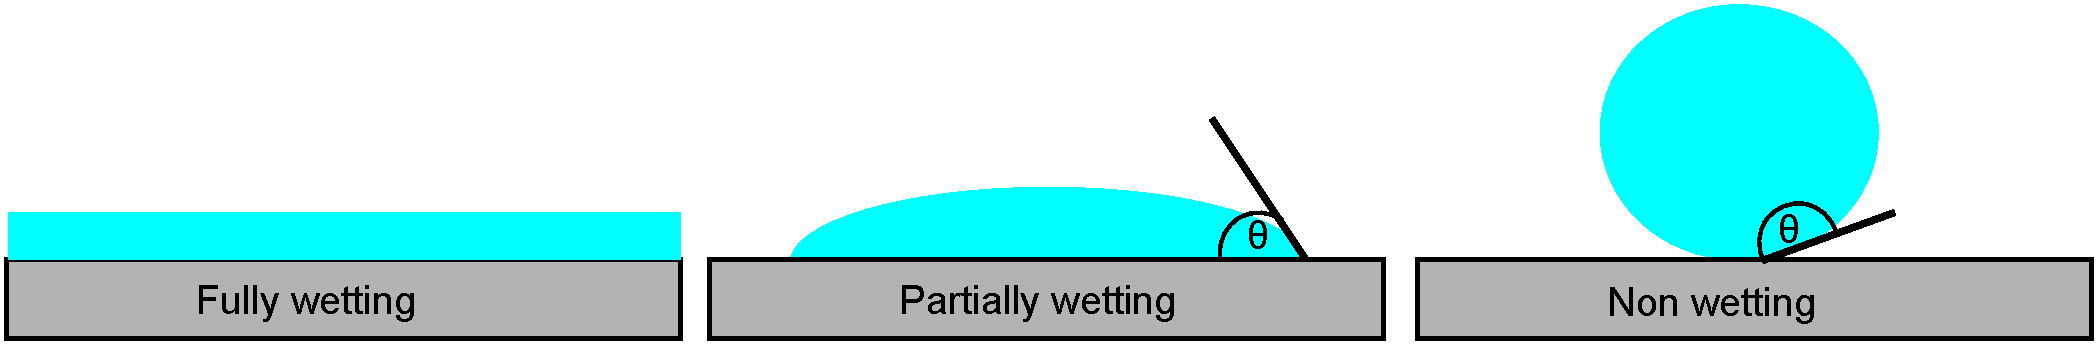
\includegraphics[width=0.95\textwidth]{graphics/Wettings.pdf}
    \caption{Wetting behaviour for different fluid substrate interactions.
    If the affinity between fluid and substrate is very large the substrate is said to be fully wetting with a vanishing contact angle.
    Reducing this affinity, which is usually the case for real substrates, leads to a measurable contact angle and is called partially wetting.
    Surface treatment or complex surface structure can lead to non wetting surfaces, therefore with contact angles of close to $\pi$.}
    \label{fig:wetting_angle}
\end{figure} 

In contrast to the previous section we started this section with the result the thin film equation.
What follows now is the derivation of Eq.~(\ref{eq:simple_thin_film}) from the Navier-Stokes equation.

\subsection{Scaling and boundary conditions}
\label{subsec:thin_film_scaling}
Thin liquid films are \textit{thin}, i.e., there is always a spatial dimension which is much smaller than the other ones. 
Some instructive everyday example that enforces this understanding would be the thickness of an oil film in a frying pan. 
The pan is about 30cm in diameter while the thickness of the oil film is not even 1cm.
Assuming that the oil is covering the whole surface of the pan $\varepsilon < 10^{-1}$.
While this example is very illustrative it also displays interesting physics.
When the pan is heated the film usually ruptures in the middle and a ring-like structure is left as shown in Ref.~\cite{fedorchenkoFormationDrySpots2021}.

The basic assumption is, again, the absence of strong slopes and therefore
\begin{equation}\label{eq:small_slopes}
    |\nabla h| \ll 1,  
\end{equation}
meaning that the thickness changes gradually along the two horizontal dimensions.

Before we start the derivation we rescale length and velocity components to have dimensionless quantities.
We use a similar scaling as in Eq.~(\ref{eq:thickness_length}) and get 
\begin{align}\label{eq:thin_film_scaling}
    \tilde{x} &= \frac{x}{L},\quad \tilde{y} = \frac{y}{L},\quad \tilde{z} = \frac{z}{H},\nonumber \\
    \tilde{u}_x &= \frac{u_x}{U},\quad \tilde{u}_y = \frac{u_y}{U},\quad \tilde{u}_z = \frac{u_z}{V},\nonumber \\
    \tilde{t} &= \frac{L}{U} t,\quad \tilde{p} = \frac{H^2 p}{\mu U L}, 
\end{align}
where $U$ and $V$ are characteristic velocities and $L$ and $H$ are characteristic length scales in horizontal and vertical dimension.
The scaling factor in front of the pressure can be calculated assuming stationary unidirectional flow with $\mathbf{u} = (u(z), 0, 0)$.
It is this scaling factor ($\mu U L /H^2$) that requires that inertial effects are small and $Re<1$.
In many applications the small Reynolds number limit is a good approximation, however for e.g., spin coating inertia is not negligible.
To account for inertial effects the scaling, Eq.~(\ref{eq:thin_film_scaling}), must be modified. 
For example the pressure scaling would change to $p = \rho U^2\tilde{p}$~\cite{crasterDynamicsStabilityThin2009}.

In the shallow water section, we quickly reduced the problem to two dimensions (one horizontal and one vertical).
Here we keep the second horizontal dimension ($\tilde{y}, \tilde{u}_y$), because most numerical experiments in Chaps.~\ref{chapter:fourth_paper}-\ref{chapter:third_paper} are computed in a two dimensional domain. 
 
The first step in the derivation is to insert the dimensionless variables into the continuity equation, Eq.~(\ref{eq:incomp})
\begin{equation}\label{eq:cont_thin_film_1}
     \vec{\nabla}\cdot\vec{u} = \partial_{\tilde{x}} \tilde{u}_x + \partial_{\tilde{y}} \tilde{u}_y + \frac{V L}{U H}\partial_{\tilde{z}} \tilde{u}_z = 0,
\end{equation}
which means that $V = U H/L$ to ensure all terms are of the same order in $\varepsilon$.
Upon inserting them into the Navier-Stokes equation for the x-component only we get
\begin{align}
     \rho L \partial_{\tilde{t}}\tilde{u}_x &+ \rho\left[\frac{U^2}{L}\left(\tilde{u}_x\partial_{\tilde{x}}\tilde{u}_x + \tilde{u}_y\partial_{\tilde{y}}\tilde{u}_x\right) + \frac{U V}{H}\tilde{u}_z\partial_{\tilde{z}}\tilde{u}_x\right] = \nonumber \\ &-\frac{\mu U}{H^2} \partial_{\tilde{x}} \tilde{p} + \mu\left[\frac{U}{L^2}(\partial^2_{\tilde{x}}\tilde{u}_x + \partial^2_{\tilde{y}}\tilde{u}_x) + \frac{U}{H^2}\partial^2_{\tilde{z}}\tilde{u}_x\right].
\end{align}
For the $y$ and $z$ component we refer to the review by Oron et al.~\cite{oronLongscaleEvolutionThin1997}.
Although the equation is now non-dimensional it is instructive to multiply both sides with $H^2/\mu U$ and collect the characteristic quantities in dimensionless numbers, here the Reynolds number $Re = (\rho H U)/\mu$, see Eq.~(\ref{eq:Re_and_Fr}), and $\varepsilon$  
\begin{equation}
    \varepsilon Re \left(\partial_{\tilde{t}}\tilde{u}_x + \tilde{u}_x\partial_{\tilde{x}}\tilde{u}_x + \tilde{u}_y\partial_{\tilde{y}}\tilde{u}_x + \tilde{u}_z\partial_{\tilde{z}}\tilde{u}_x \right) = -\partial_{\tilde{x}}\tilde{p} + \varepsilon^2\left(\partial^2_{\tilde{x}}\tilde{u}_x + \partial^2_{\tilde{y}}\tilde{u}_x\right) + \partial^2_{\tilde{z}}\tilde{u}_x. 
\end{equation}
By definition $\varepsilon$ is small and terms with higher order in $\varepsilon$ are at most subleading.
Collecting only the term of $O(1)$ and performing the same scaling for the two other directions leads to the non-dimensional momentum equation of a thin film on a solid substrate
\begin{align}
    -\partial_{\tilde{x}}\tilde{p} + \partial^2_{\tilde{z}}\tilde{u}_x &= 0,  \label{eq:thin_film_pressure_x}\\
    -\partial_{\tilde{y}}\tilde{p} + \partial^2_{\tilde{z}}\tilde{u}_y &= 0,  \label{eq:thin_film_pressure_y}\\
    \partial_{\tilde{z}}\tilde{p} &= 0. \label{eq:thin_film_pressure_z}
\end{align}
For the last of the above equations the analogy to the shallow water model can be drawn using Eq.~(\ref{eq:hydrostat_sw_euler}) which states that the pressure gradient does not depend on $z$.
 
The system so far does not resemble Eq.~(\ref{eq:simple_thin_film}).
Therefore, some more derivation is in order, starting with the application of the boundary conditions.
Between the fluid and solid phase a no-slip boundary condition is used. 
Similar to Eq.~(\ref{eq:no-slip_sw1}) and~(\ref{eq:no-slip_sw2}) we have
\begin{equation}\label{eq:thin_all_v_noslip}
    \mathbf{u}|_{z=0} = \mathbf{0},    
\end{equation}
and for the vapour fluid interface a stress balance needs to be satisfied~\cite{lealAdvancedTransportPhenomena2007}
\begin{equation}\label{eq:thin_film_upper_bc}
    (\tilde{\sigma}_l - \tilde{\sigma}_v)\cdot\mathbf{n} + \nabla_S\gamma - \gamma\mathbf{n}(\nabla\cdot\mathbf{n}) = 0,
\end{equation}
% I am here
where $\tilde{\sigma}_{l,v}$ are the stress tensors for the liquid ($l$) and the vapour ($v$) phase. 
Furthermore, we have the normal vector $\mathbf{n}$ along the fluid interface and the surface gradient $\nabla_S$.
The two surface tension terms account for changes along the surface ($\nabla_S$) and the Laplace pressure due the curvature ($\kappa$) of the liquid vapour interface $2\kappa = \nabla\cdot\mathbf{n}$.
The stress tensor for a Newtonian liquid has been defined in Eq.~(\ref{eq:total_stress}) and for the sake of completeness it is given in matrix notation as 
\begin{gather}\label{eq:stress_matrix}
    \tilde{\sigma} = \begin{bmatrix}
    -p + 2\mu\partial_x u_x & \mu(\partial_y u_x + \partial_x u_y) & \mu(\partial_z u_x + \partial_x u_z) \\
    \mu(\partial_x u_y + \partial_y u_x) & -p + 2\mu\partial_y u_y & \mu(\partial_z u_y + \partial_y u_z) \\
    \mu(\partial_x u_z + \partial_z u_x) & \mu(\partial_y u_z + \partial_z u_y) & -p + 2\mu\partial_z u_z   
    \end{bmatrix} .
\end{gather}
The normal vector $\mathbf{n}$ along the interface is defined as 
\begin{equation}\label{eq:normal_vec_thin_film}
    \mathbf{n} = \frac{1}{\sqrt{1 + (\partial_x h)^2 + (\partial_y h)^2}}(-\partial_x h, -\partial_y h, 1).
\end{equation}
Computing the inner product of Eq.~(\ref{eq:thin_film_upper_bc}) with the normal vector $\mathbf{n}$ yields
\begin{equation}\label{eq:balance_stresses_normal}
    p_v - p -(\mathbf{n}\cdot\mathbf{T})\cdot\mathbf{n} + \gamma\mathbf{n}(\nabla\cdot\mathbf{n})\cdot\mathbf{n} = 0,
\end{equation}
where $p_v$ is the pressure in the vapour phase and $\mathbf{T} = \mu(\nabla\mathbf{u} + \nabla\mathbf{u}^T)$.
In fact only the contribution from the liquid is considered, because $\mu_l \gg \mu_v$.
Assuming a water/air interface (which is not too different from a water/water vapor interface) we have a ratio of dynamic viscosity $\mu_{air} / \mu_{\ce{H2O}} = 0.018~mPa\cdot s/ 1.0016~mPa\cdot s \approx 0.02$.
Inserting the scaling defined in the Eq.~(\ref{eq:thin_film_scaling}) and collecting only leading order contributions we have 
\begin{equation}
    \tilde{p} = p_v + P - \gamma(\partial_{\tilde{x}}^2 h + \partial_{\tilde{y}}^2 h),
\end{equation}
where $P$ accounts for all additional contributions to the pressure, e.g., the hydrostatic pressure, see for example Eq.~(\ref{eq:hydro_static_int}), but as well for the disjoining pressure $\Pi(h)$ Eq.~(\ref{eq:disj_pressure_one}).

Now that the normal stresses are balanced at the fluid vapour interface the same has to be done for the tangential stresses.
Again we use Eq.~(\ref{eq:thin_film_upper_bc}) and compute the inner product with the tangential unit vectors $\mathbf{t}_i$ 
\begin{equation}\label{eq:upper_bc_tangential}
    \mathbf{t}_i(\mathbf{T}_l - \mathbf{T}_v)\cdot\mathbf{n} + \mathbf{t}_i\cdot\nabla_S\gamma = 0.
\end{equation}
The high viscosity contrast between the liquid and vapour allows us to neglect contributions from $\mathbf{T}_v$.
Collecting leading order terms we have
\begin{align}
    \mu\partial_{\tilde{z}}\tilde{u}_x = \tau_x, \label{eq:tau_x_thin}\\
    \mu\partial_{\tilde{z}}\tilde{u}_y = \tau_y. \label{eq:tau_y_thin}
\end{align}
Having defined the leading order equations for the flow velocity, the next step is to integrate them along the vertical dimension.

\subsection{Vertical integration}
\label{subsec:thin_film_int}
The system of equations so far do not resemble Eq.~(\ref{eq:simple_thin_film}).
To get to Eq.~(\ref{eq:simple_thin_film}) we still need to perform the integration along the vertical dimension.
Dropping the tilde for now as all variables are dimensionless we have, 
\begin{align}\label{eq:int_vels_thin}
    \iint (-\partial_x p + \partial_z^2 u_x ) \diff^2 z = 0,  \\
    \iint (-\partial_y p + \partial_z^2 u_y ) \diff^2 z = 0. 
\end{align}
From Eq.~(\ref{eq:thin_film_pressure_z}) we know that the pressure gradient is conserved along $z$. 
Therefore integrating Eqs.~(\ref{eq:thin_film_pressure_x}, \ref{eq:thin_film_pressure_y}) twice with respect to $z$ yields
\begin{align}
    u_x = \frac{\partial_x p}{2\mu}(z^2 - 2hz) + \frac{\tau_x z}{\mu}, \label{eq:vel_x_int_thin}\\
    u_y = \frac{\partial_y p}{2\mu}(z^2 - 2hz) + \frac{\tau_y z}{\mu}, \label{eq:vel_y_int_thin}
\end{align}
where we used Eqs.~(\ref{eq:thin_all_v_noslip}, \ref{eq:tau_x_thin}, \ref{eq:tau_y_thin}) to determine the integration constants.
In the following, many steps are fairly similar to the derivation of Sec.~\ref{sec:theory_shallow_water}, however, it is instructive to proceed step by step.
Performing another integration of the velocities with respect to the thickness to compute the discharge $Q$ or volume flux 
\begin{align}
    Q_x = \int_0^h u_x(z)\diff z = -\frac{h^3}{3\mu}\partial_x p + \frac{h^2}{2\mu} \tau_x, \label{eq:discharge_thin_x} \\
    Q_y = \int_0^h u_y(z)\diff z = -\frac{h^3}{3\mu}\partial_y p + \frac{h^2}{2\mu} \tau_y, \label{eq:discharge_thin_y}
\end{align}
where due to the no slip boundary condition the mobility function $M(h)$, Eq.~(\ref{eq:no-slip-mobility}) naturally arises.

Now that the horizontal velocities are known we can perform the integration of the continuity equation Eq.~(\ref{eq:incomp})
\begin{equation}\label{eq:cont_thin}
    \int_0^h(\partial_x u_x + \partial_y u_y + \partial_z u_z) = 0,
\end{equation}
making use of the Leibniz rule one more time and showing only the $x$ component
\begin{equation}
    \int_0^h \partial_x u_x(z) \diff z = \partial_x\int_0^h u_x\diff z + \partial_x 0 u_x(0) - \partial_x h u_x(h) = \partial_x Q_x - \partial_x h u_x(h),  
\end{equation}
where Eq.~(\ref{eq:discharge_thin_x}) was used.
Inserting the above equation for the $x$ and $y$-component into the Eq.~(\ref{eq:cont_thin}) and performing the integration of $\partial_z u_z$ yields
\begin{equation}\label{eq:thin_dummy}
    \partial_x Q_x - (\partial_x h) u_x(h) + \partial_y Q_y - (\partial_y h) u_y(h) + u_z(h) - u_z(0) = 0.
\end{equation}
Since the no-slip boundary condition holds for all velocity components we set $u_z(0) = 0$.
The upper bound $u_z(h)$ can be computed using the material derivative, see Eq.~(\ref{eq:mat_dev}). 
We apply the same transformation as in Eq.~(\ref{eq:shallow_water_height}) with $f(\mathbf{x},t) = h(\mathbf{x},t) - z$, which is $0$ at the interface yields
\begin{equation}\label{eq:mat_uz_h}
    D_t f = \partial_t h + u_x\partial_x h + u_y\partial_y h - u_z = 0.
\end{equation}
Inserting the found result for $u(h)$ into Eq.~(\ref{eq:thin_dummy}) we get
\begin{equation}\label{eq:thin_obsc}
    \partial_x Q_x + \partial_y Q_y + \partial_t h = 0,
\end{equation}
which is almost the same as Eq.~(\ref{eq:simple_thin_film}).
Inserting $Q_x$ and $Q_y$, Eqs.~(\ref{eq:discharge_thin_x}) and (\ref{eq:discharge_thin_y}), we have
\begin{equation}
    \partial_t h(\mathbf{x},t) = \nabla\cdot\left(\frac{h^3}{3\mu}\nabla p + \frac{h^2}{2\mu}\tau\right),
\end{equation}
which in contrast to Eq.~(\ref{eq:simple_thin_film}) includes the shear contribution $\tau$.
Assuming the interface is not accelerated (e.g., in case of dewetting) the shear term can be neglected and the resulting equation is 
\begin{equation}\label{eq:thin_final}
    \partial_t h(\mathbf{x},t) = \nabla\cdot\left(\frac{h^3}{3\mu}\nabla p\right),
\end{equation}
which completes the task to derive the thin film equation from the Navier-Stokes equation. 
To sum up the approach in one sentence, we non dimensionalized the variables, collected terms in orders of $\varepsilon$, used our boundary conditions and performed an integration along the vertical dimension to average out the vertical dynamics.
Of course this derivation comes short if there are additional forces to consider such as thermal fluctuations, that said in Chap.~\ref{chapter:second_paper} we discuss the effect of thermal fluctuations on dewetting and show how the thin film equation has to be modified.

Because the thin film equation is the main theoretical framework for the following Chaps. it is instructive to derive some more phenomenology of Eq.~(\ref{eq:thin_final}).
One helpful tool is the so called linear stability analysis. 
The idea is to slightly perturb the system, Eq.~(\ref{eq:thin_final}), and derive its response to the pertubation.

\subsection{Linear stability analysis}
\label{susbsec:Lin_stab}
The concept of the linear stability analysis is a rather interesting one.
One takes a stable solution of a mathematical system, in our case the thin film equation, and perturbs the stable solution.
Will the system come back to the stable solution and therefore damp out the perturbation or will the system become unstable and open up a new branch in the phase space of solutions?

A simple example for this can be the string of a guitar.
In the rest case, which forms a stable solution for the length of the string, the string is flat.
If one gently touches the string a small perturbation is added and will undulate the string such that it starts to vibrate.
The vibrations will turn into waves with well defined wavelengths. 
Most of them will be damped and usually only one wave mode will survive.
The sound related to that wave mode defines the eigenmode of the string.
Due to friction and boundary conditions the string will go back to be flat, which means that the string is linearly stable.

Using this analysis for the thin film equation we simply add a small perturbation to a flat film with
\begin{equation}\label{eq:lin_stab_delta}
    h(\mathbf{x},t) = h_0 + \delta h(\mathbf{x},t),
\end{equation}
where $h_0$ is the thickness of the flat film and $\delta h$ is the small, but dynamic perturbation.
Small in this sense that $\delta h \ll h_0$.
Now we follow the development of the perturbation and therefore quantify the stability of the system.
The name ``linear stability analysis'' comes from the fact that one considers only terms up to $O(\delta h)$, but neglects higher orders of $\delta h$~\cite{laugesenLinearStabilitySteady2000}.

Inserting Eq.~(\ref{eq:lin_stab_delta}) into Eq.~(\ref{eq:thin_final}) yields
\begin{equation}\label{eq:stab_1}
    \partial_t (h_0 + \delta h) = \nabla\cdot\left\{\frac{(h_0 + \delta h)^3}{3\mu}\nabla [-\gamma\Delta(h_0 + \delta h) - \Pi(h_0 + \delta h)]\right\},
\end{equation}
where the pressure term has been written explicitly in terms of the Laplace and the disjoining pressure.
Using the fact that $h_0$ is constant and thus $\nabla h_0 = \partial_t h_0= 0$ we can compute the derivatives
\begin{equation}\label{eq:stab_2}
    \partial_t \delta h = \frac{h_0^3}{3\mu}\left[-\Pi'(h_0)\nabla^2\delta h -\gamma\nabla^4\delta h\right],
\end{equation}
where $\Pi'(h_0)$ is a short notation for
\begin{equation}\label{eq:deriva_Pi}
    \Pi'(h_0) = \frac{\partial\Pi(h)}{\partial h}\bigg\rvert_{h=h_0}.
\end{equation}

Instead of solving this equation in real space it is simpler to solve it in Fourier space.
This further means that a wavelength $\lambda$ in real space becomes a wavemode $q$ in Fourier space. 
Fourier transforming the perturbation $\delta h$ we have 
\begin{equation}\label{eq:fourier_h}
    \tilde{\delta h}(\mathbf{q},t) = \int_{-\infty}^{\infty} \delta h(\mathbf{x},t) e^{-i\mathbf{x}\cdot\mathbf{q}} \diff\mathbf{x}.    
\end{equation}
Under the Fourier transformation the derivatives become wavevectors ($\mathbf{q}$) and Eq.~(\ref{eq:stab_2}) reads
\begin{equation}\label{eq:stab_3}
    \partial_t \tilde{\delta h}(\mathbf{q},t) = \frac{h_0^3}{3\mu}\left[-\Pi'(h_0)\mathbf{q}^2\delta h -\gamma\mathbf{q}^4\delta h\right].
\end{equation}
From the above equation one can readily read the dispersion relation $\omega(q)$ as 
\begin{align}
    \partial_t \tilde{\delta h} &= \omega(q)\tilde{\delta h}, \\
    \omega(q) &= \frac{h_0^3}{3\mu}\left[-\Pi'(h_0)q^2 -\gamma q^4\right], 
\end{align}
where $q = \sqrt{q_x^2 + q_y^2}$.
To find the fastest growing unstable wavemode $q_0$ which is also called the eigenmode of the (spinodally dewetting) film we set the left hand side equal to $0$ and solve for $q$
\begin{align}\label{eq:stab_4}
    \partial_t \tilde{\delta h} &= 0, \\
    \frac{h_0^3}{3\mu}q^2\left[-\Pi'(h_0)\delta h -\gamma q^2\delta h\right] &= 0, \\
    -\Pi'(h_0) -\gamma q^2 &= 0, \\
    q_0 &= \sqrt{\frac{-\Pi'(h_0)}{\gamma}} .
\end{align}

An example of a dispersion relation which follows the above equation is shown in Fig.~\ref{fig:dispertion_1}.
In this figure we can identify two relevant wave numbers, on the one hand there is $q_0$ which is the fastest growing mode indicated by a dotted line and there is $q_m = \sqrt{2}q_0$ which is the largest wave number that is not damped.
Wavemodes larger than $q_m$ are therefore damped out.
A characteristic time scale of the problem is given as
\begin{equation}
    t_0 = \frac{3\mu}{\gamma h_0^3 q_0^4},
\end{equation}
with is used to normalize the time in Fig.~\ref{fig:dispertion_1}.
Because the concept of linear stability is such an important one, we encounter it again in Chap.~\ref{chapter:first_paper} (see Fig.~\ref{fig:RTI}) as well as in Chap.~\ref{chapter:second_paper} (see Figs.~\ref{fig:theory_simulation_structure_factor}, \ref{fig:spectral_analysis_deter_sine8}, \ref{fig:spectral_analysis_stoch_sine8}, \ref{fig:square_wave_both}).
Chap.~\ref{chapter:second_paper} focuses only on the addition of a fluctuating term and the so called stochastic thin film equation.
The new term due to thermal fluctuations offers some interesting features on both the structure factor as well as the dispersion.

\begin{figure}
    \centering
    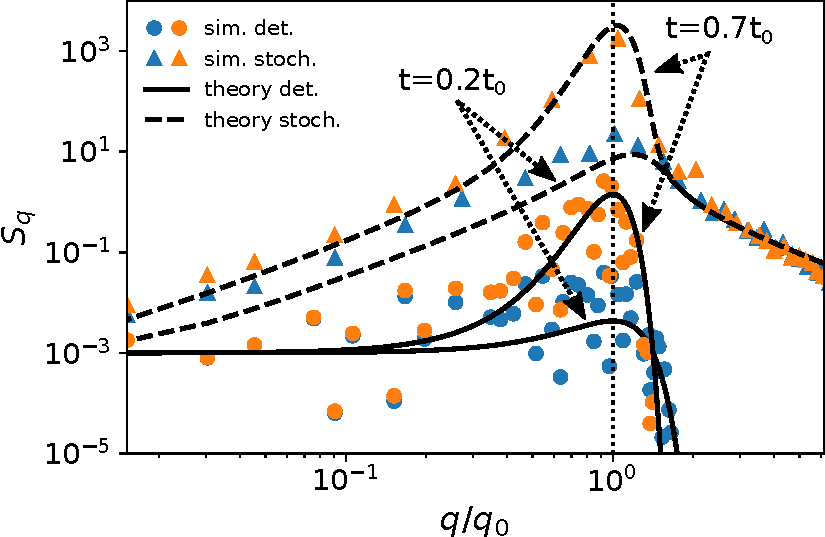
\includegraphics[width=0.65\textwidth]{graphics/spectratheta20.pdf}
    \caption{Dispersion relation of a spinodally dewetting thin film with and without thermal fluctuations.
    Where $S(q)$ is the structure factor depending on the wavemode $q$.
    The dots and triangles are generated using the here presented numerical method. 
    Full and dashed lines are the theoretical prediction based on Eq.~(\ref{eq:simple_thin_film}) and its fluctuating extension, Eq.~(\ref{eq:structure_factor_2}).
    }
    \label{fig:dispertion_1}
\end{figure}

\section{Differences and overlap}
\label{sec:shallow_to_thin}
The theoretical starting point of this chapter is the Navier-Stokes equation.
This equation relates the change of momentum of the fluid to various effects, e.g., viscous contributions. 
As of today, nobody has solved the Millennium Problem and proven that there exist a unique and smooth solution to this equation.
A well defined solution would have the benefit that even complex flow fields could be computed using analytical methods, such as pen and paper.
What we can do, is computing approximative results of this equation using numerical techniques.
This is in fact the idea of the following chapter.
Mathematically the incompressible Navier-Stokes equation is a second order partial differential vector equation. 
It can be considered hyperbolic if the flow is advection dominated or parabolic if it is diffusion dominated.
The Reynolds number is the one dimensionless number that helps to distinguish between these two regimes. 

For many flows we actually do not need to solve the Navier-Stokes equation.
In Sec.~\ref{sec:theory_shallow_water} we introduce the concept of dimensional reduction by integrating out the horizontal degrees of freedom.
This reduction is build on the fact that we consider two length scales, a vertical and horizontal scale, with a scaling parameter $\varepsilon$. 
Applying this scaling and collect terms in orders $O(\varepsilon)$ we derive a different continuity and momentum equation, see Eqs.~(\ref{eq:shallow_water_01}-\ref{eq:shallow_water_02}).
We exchange the fluid density $\rho(\mathbf{x},t)$ for a fluid ``height'' $h(\mathbf{x},t)$, which is measured from the bottom topography to the fluid/vapour interface.
The resulting set of equations, Eqs.~(\ref{eq:shallow_water_01}-\ref{eq:shallow_water_02}), are hyperbolic partial differential equations.
Assuming that $\mathcal{S}$ in Eq.~(\ref{eq:shallow_water_02}) is a Newtonian viscous stress analogue to Eq.~(\ref{eq:stress_tens}) we have a second order vector equation in $(h, u_x, u_y)$.  
The shallow water equations cover a wide ranges of geophysical flow problems, from slowly creeping lava to quickly evolving weather systems.
At no point in the derivation of the theory we required that dimensionless numbers, such as the Reynolds number, are small or vanishing. 
In fact it is straightforward to derive the inviscid shallow water equations for large Reynolds numbers. 
An interesting phenomenon that can be explained with the inviscid shallow water equations are soliton like solutions.
These solutions are stable travelling waves with a constant velocity and no dispersion, famous examples are tsunamis and river bora.
One word of caution these solutions are valid in ``open'' water, as soon as these waves come close to shore the breaking wave dynamics cannot be explained with the simple set of equations we derived here. 
In most of the shallow flows considered here the fluid viscosity is at most subleading.
This does not mean that there are no models considering viscosity, see for example Ref.~\cite{marcheDerivationNewTwodimensional2007}.
The main source of friction and thus dissipation is however the interaction with the bottom topography, we for example required that the flow velocity vanished at $z = -h(x,y)$.
Lastly, in our derivation we did not consider surface tension as a leading order contribution to the shallow water equations.
The shape of the fluid/vapour interface is driven by the hydrostatic pressure.

The last model we introduce in this chapter is the thin film equation, Eq.~(\ref{eq:thin_final}). 
In Sec.~\ref{sec:thin_films} we start with a discussion on the phenomenology of thin film flows and peculiarities of modelling wetting and contact line dynamics.
If we leave aside the disjoining pressure $\Pi(h)$, see Eq.~(\ref{eq:disj_pressure_one}), and only consider the capillary pressure ($\Delta h$), the thin film equation is a degenerate, fourth order parabolic partial differential equation of the film thickness $h(\mathbf{x},t)$~\cite{peschkaVariationalApproachDynamic2018}.
In contrast to the shallow water equations and the Navier-Stoke equation, the thin film equation is a single scalar equation.
Therefore there is no momentum equation, but only a continuity equation for the film thickness.
The thin film equation is a highly non-linear equation similar to both the Navier-Stokes and the shallow water equations. 
One example for these non-linearities is the dynamics of droplet formation after rupture of an unstable thin film. 
The equation allows for many instabilities such as fingering, tearing and pearling~\cite{crasterDynamicsStabilityThin2009, wilczekSlidingDropsEnsemble2017}. 
The steps to derive the thin film equation are in parts similar to the shallow water system.
Starting with a rescaling of the continuity equation, Eq.~(\ref{eq:incomp}), and the Navier-Stokes equation, Eq.~(\ref{eq:navier_stokes_fin}) (with $\mathbf{F} = 0$) and assuming that one dimension is much smaller than the others. 
However, in contrast to the shallow water system this scaling ansatz we choose is only suitable for negligible inertial contributions.
Terms are then collected in orders of $\varepsilon$ similar to the shallow water derivation.
The boundary condition at $z=0$ is another shared feature between the shallow water equations and the thin film equation, at least for the no-slip mobility Eq.~(\ref{eq:no-slip-mobility}).
If we relax this boundary condition, which is the case in the following chapters, then we introduce a so-called slip length which is not accounted for in the shallow water equations.
The stress balance at the liquid/vapour interface is another difference between the shallow water equation and the thin film equation, for the normal stress component we have Eq.~(\ref{eq:thin_film_upper_bc}).
We have another balance equation for the tangential stress with Eq.~(\ref{eq:upper_bc_tangential}).
Balancing the surface stresses also introduces the surface tension, a contribution that keeps the liquid/vapour interface minimal.  
To reduce the dimensionality of the problem we perform an integration along the vertical direction, similar to the shallow water derivation.
In the last step we use the material derivative, Eq.~(\ref{eq:mat_dev}), to compute a relation between the flow velocity at the liquid/vapour interface and the discharge $\mathbf{Q}$.
Because of Eqs.~(\ref{eq:discharge_thin_x}-\ref{eq:discharge_thin_x}) we know that the discharge is pressure dependent, and thus we end up with Eq.~(\ref{eq:thin_final}).
The velocities are therefore effectively captured by a pressure gradient and if applicable a shear rate $\tau$.

While there are many similarities between the thin film equation and the shallow water equations, there are also some major differences.
The most pressing difference between these two models is the fact that the shallow water equation is a vector equation while the thin film equation is a scalar equation.
In the shallow water equations the liquid/vapour interface is driven by hydrostatic pressure while in the thin film equation we neglect the hydrostatic pressure and introduce surface tension and capillarity.
The question that naturally arise here is: can one model be translated into the other one?
Although this question seems odd at first it is actually of great significance to show that problems can be solved with different approaches.
There are several numerical methods to iteratively solve the thin film equation.
There are as well several different numerical methods to approximate the Navier-Stokes equation.
The important contribution to our understanding of CFD is that methods build to solve the shallow water equations can actually be used to solve the thin film problem, as discussed in Chap.~\ref{chapter:first_paper}